% Created 2023-10-25 Wed 15:53
% Intended LaTeX compiler: pdflatex
\documentclass[11pt]{article}
\usepackage[utf8]{inputenc}
\usepackage[T1]{fontenc}
\usepackage{graphicx}
\usepackage{longtable}
\usepackage{wrapfig}
\usepackage{rotating}
\usepackage[normalem]{ulem}
\usepackage{amsmath}
\usepackage{amssymb}
\usepackage{capt-of}
\usepackage{hyperref}
\usepackage{graphicx}
\graphicspath{ {./images/} }
\author{Hankertrix}
\date{\today}
\title{Genetic Diversity Cheat Sheet}
\hypersetup{
 pdfauthor={Hankertrix},
 pdftitle={Genetic Diversity Cheat Sheet},
 pdfkeywords={},
 pdfsubject={},
 pdfcreator={Emacs 29.1 (Org mode 9.6.6)}, 
 pdflang={English}}
\begin{document}

\maketitle
\setcounter{tocdepth}{2}
\tableofcontents

\newpage

\section{Definitions}
\label{sec:org0c1d8cf}

\subsection{Genetic diversity}
\label{sec:org0c67da8}
Genetic diversity refers to the state where genetic variations are numerous within the population of a species. It is \textbf{not} genetic diversity if comparing across genetic variations of only two or three individuals, as they are simply variants of each other.
\\[0pt]

Populations with high genetic diversity are more likely to have some individuals that can survive a significant change in their environment. If a species' population is small and isolated, it is more likely to become extinct due to a limited genetic diversity.
\\[0pt]

For example, green frogs have traits that cause them to be unable to survive a natural disaster. In the event of a natural disaster, the entire population of frogs will be killed off if it only consists of green frogs, which will lead to extinction. As such, genetic diversity is very important in a population.

\subsection{Alleles}
\label{sec:org6ed9874}
Alleles are variants of a gene.

\subsection{Genotype}
\label{sec:org631b4d4}
Genotype refers to the genetic constitution of living organisms. It is the total sum of genes transferred from parents to offspring. It can also be defined as the complete set of heritable genes that can be transferred to the offspring from its parents.

\subsection{Phenotype (Character)}
\label{sec:orga6615dc}
Phenotype refers to the observable physical properties of an organism.

\subsection{Trait}
\label{sec:org2f74e89}
A trait is an expression of a character (phenotype).

\subsection{Heredity}
\label{sec:orgf7835ab}
Heredity is the tendency for traits to be passed from parents to offspring. In genetic studies, we often aim to associate hereditary basis (alleles of genes, genotype) to a particular trait (phenotype).

\subsection{Classical genetics (Mendelian genetics)}
\label{sec:org6b5d50e}
Classical genetics that look at crosses or relationship of alleles in such a manner (dominant or recessive) are therefore, referred to as Mendelian genetics or inheritance.
\\[0pt]

Before the discovery of DNA and chromosomes, principles of heredity were worked out by quantitative science, i.e. counting and measuring. Classical genetics is the statistics of the phenotypes of offspring.
\\[0pt]

Gregor Mendel established the method and principles of classical genetics, and hence, classical genetics is sometimes referred to as Mendelian genetics.

\subsection{Homozygote (plural: homozygous)}
\label{sec:org2fa06d7}
Homozygote refers to an organism which has two \textbf{identical} alleles of a particular gene or genes.

\subsection{Heterozygote (plural: heterozygous)}
\label{sec:orgbe1b16f}
Heterozygote refers to an organism which has two \textbf{different} alleles of a particular gene or genes.

\newpage

\subsection{Punnett square}
\label{sec:org304e1e7}
A Punnett square is a square diagram that is used to predict the genotypes of a particular cross or breeding experiment.

\[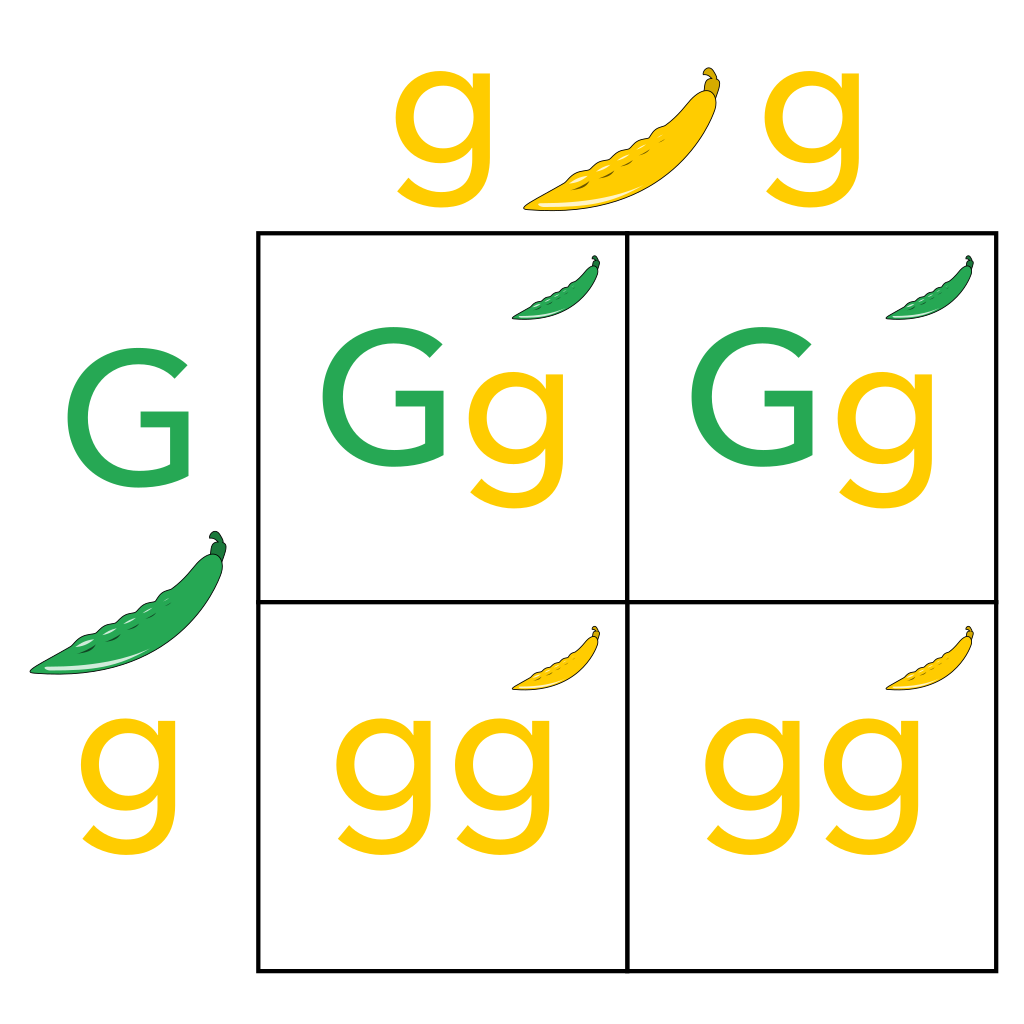
\includegraphics[scale = 0.2]{punnett-square}\]

\subsection{Mendel's first law: segregation}
\label{sec:orgb9f45c8}
The two alleles of a trait separate from each other during the formation of gametes, so that half of the gametes will carry one copy, and half will carry the other copy.

\subsection{Mendel's second law: independent assortment}
\label{sec:orgccc0b8b}
Genes located on different chromosomes are inherited independently of one another.

\subsection{Dihybrid}
\label{sec:org75e64b0}
A dihybrid individual is an individual that has two \textbf{different} alleles for each of the two traits being investigated.

\subsection{Pleiotropic alleles}
\label{sec:org63f9f71}
Pleiotropic alleles refer to alleles that have more than one effect on a phenotype.

\subsection{Molecular genetics}
\label{sec:org17b4b00}
Molecular genetics adopts the understanding of DNA at the molecular level to examine inherited traits. In very recent years, this has also led to a leap in technology to give rise to the field of "genomics" and other "-omics".

\subsubsection{Differences from Mendelian genetics}
\label{sec:orga310914}
Mendelian traits rely on what can be observed at the organism level, like if the person is anaemic.
\\[0pt]

Molecular genetics may rely on observations at either the primary transcript, messenger RNA or polypeptide level to distinguish between phenotypes, such as misfolded proteins or the lack of mRNA produced. Molecular genetics allow the "why" or "how" of phenotypic variation to be deciphered through analysis of the DNA sequence, like if the variant had a substitution resulting in a change in amino acid sequence.
\\[0pt]

This means that in molecular genetics, the following levels of analysis can be used to identify the phenotypes presented by any one allele of a gene:
\begin{itemize}
\item mRNA transcript level
\item Quantity of protein expressed
\item Variation in activity or the quality of the protein
\end{itemize}

In molecular genetics, it is also possible to study the phenotypes presented by both alleles of a homologous pair by analysis at the cellular level. For example, a cell of a particular genotype may have a modified cell shape, or grows slower, due to the combined effects of the two alleles.

\newpage

\subsubsection{The molecular genetics approach}
\label{sec:orgf613208}
We can use a combination of DNA manipulation techniques to find out:
\begin{itemize}
\item Where the gene responsible may be located.
\item What sequence change caused the phenotype to change.
\end{itemize}

If the phenotypic difference is known, then DNA analysis can be carried out to figure out where the gene responsible for the phenotypic difference is located.
\\[0pt]

If the sequence difference is known, but the phenotypic difference is not known, then observation of the phenotypic difference will reveal the function of the gene that has changed.

\subsection{Evolution}
\label{sec:org46bde38}
Evolution is the unifying principle of biology. Evolution explains the unity (commonality and diversity of life).
\begin{itemize}
\item Similarities between living things reflect \textbf{recent} common ancestry
\item Dissimilarities between living things reflect \textbf{ancient} common ancestry
\end{itemize}

This similarity and dissimilarity exists not only at the level of observable traits, but also at the molecular level.
\begin{itemize}
\item The DNA sequence of genomes can be compared to trace the commonality of ancestry of several organisms.
\item The amino acid sequence of proteins can be compared to trace the commonality of ancestry of a specific protein that can be found in several organisms.
\end{itemize}

Essentially, by taking samples to be compared in the present day, we can trace their relationship in the past through the evolutionary tree.

\newpage

\subsection{Natural selection (survival of the fittest)}
\label{sec:orgb3513e0}
Natural selection is a process described as such:
\begin{enumerate}
\item Members of a population have inheritable variations.
\item More individuals are produced in each generation than the environment can support.
\item Some individuals have adaptive characteristics, which are favourable traits that result in increased survival and reproduction.
\item This results in an increasing proportion of succeeding generations having favourable characteristics, and results in a population adapted to the environment.
\end{enumerate}

\subsection{Darwin's theory of evolution}
\label{sec:orge7a5126}
Darwin emphasised that individuals from a population vary in their functional characteristics, physical characteristics and behavioural characteristics. He also proposed that these variations:
\begin{itemize}
\item Occur randomly
\item Are essential to the natural selection process
\item Allow adaptation of the population to the environment over time
\end{itemize}

\subsection{Fitness (Darwinian fitness)}
\label{sec:org8649de9}
Fitness is the relative reproductive success of an individual. It does not always refer to the biggest or the strongest. The most-fit individuals in a population capture a disproportionate share of goodies. Interactions with the environment determine which individuals reproduce the most.
\\[0pt]

Another way to put it is that fitness refers to organisms which survive more often and hence leave more offspring in a particular environment.

\subsection{Adaptation}
\label{sec:org0bcd324}
Adaptation is referring to the consequence of those reproductive successes to a population. Adaptation is the change that helps a species become more suited to its environment. Adaptation is a product of natural selection and is not a one-off response to environmental changes.

\subsection{Niche}
\label{sec:orge180de7}
A niche represents how a species interacts both biologically and physically with its environment in order to survive.

\subsection{Adaptive radiation}
\label{sec:org660be7c}
In adaptive radiation, a cluster of species changes to occupy a series of different habitats within a region. Each habitat offers different niches to occupy, and each species evolves to become adapted to that niche.

\subsection{Fossils}
\label{sec:org03adceb}
Fossils are the preserved remains, tracks or traces of once-living organisms. They are created when organisms become buried in sediment. By dating the rocks in which the fossils occur, one can get an accurate idea of how old the fossils are.
\\[0pt]

Fossils in rocks can represent a history of evolutionary change as fossils are treated as samples of data and are dated independently without bias from how the samples appear. Successive changes through time, as projected by the fossil record are "data statements" demonstrating that evolution has occurred.

\subsection{Homologous structures}
\label{sec:org96569e6}
Homologous structures are anatomically similar structures that are inherited from a common ancestor. They can be either functionally similar or not functionally similar.

\subsection{Analogous structures}
\label{sec:org75fa35e}
Analogous structures are structures that serve the same function but are not constructed similarly. They hence do not share a common ancestor.

\subsection{Vestigial structures}
\label{sec:org5c80af9}
Vestigial structures are fully developed anatomical structures in a group of organisms. However, these structures are reduced, or obsolete in function.

\subsection{Anatomical record}
\label{sec:orgc0f3b04}
The anatomical record is a record of the anatomy of various organisms. It also reflects evolutionary history. For example, all vertebrate embryos share a basic set of developmental instructions. This high level of similarity, for such a complex process, suggests that they have common ancestry fairly recently in evolutionary history.
\\[0pt]

We also look at homologous, analogous and vestigial structures as evidence for evolution.

\subsection{Traditional applied genetics}
\label{sec:org5a48fb8}
Traditional applied genetics refers to the selection of "parents" with the desired characteristics to create more offspring with the desired characteristics. However, the efficiency of traditionally applied genetics is not very high as the genes are unavoidably shuffled during meiosis and fertilisation. This results in only a few offspring having the desired combination of characteristics which is counter-productive to the motive behind artificial selection.

\subsection{Molecular biotechnology}
\label{sec:org44088e1}
Molecular biotechnology aims to eliminate the randomness of traditional applied genetics and is used to engineer the exact changes in genes to bring about the desired characteristics in organisms. "Molecular" refers to biomolecules like DNA, RNA and proteins. It used to be called "genetic engineering" but it is now called molecular biotechnology to reflect the diversity of techniques included in the process.

\subsection{Cloning}
\label{sec:org9351082}
Cloning is the production of identical copies of DNA, cells, or organisms. For example, a population of bacteria produced after several rounds of binary fission are clones, because they all came from division of the same cell. Identical twins are clones is they are a single embryo separating to become two.

\subsection{Gene (DNA) of interest}
\label{sec:orgd717e3c}
A gene (DNA) of interest is a gene that is cloned. It is sometimes called the insert or foreign DNA.

\subsection{Recombinant DNA}
\label{sec:org863bf5a}
Recombinant DNA contains DNA from two or more different sources.

\subsection{Vector (vector DNA)}
\label{sec:orgbaa88cc}
A vector is a piece of DNA that introduces recombinant DNA into a host cell.

\subsection{Plasmids}
\label{sec:org1941af4}
Plasmids are small accessory rings of DNA from bacteria. They are usually used as vector DNA.

\subsection{Sticky ends}
\label{sec:orgaca0737}
Sticky ends are the short single-stranded segments that result from the cleaving of DNA by a restriction enzyme. They are called "sticky" as the ends can be complementarily bonded by another compatible DNA fragment.

\subsection{Transformation}
\label{sec:orge155184}
Transformation is the process where the foreign DNA enters a host cell.

\newpage

\subsection{Gene cloning}
\label{sec:orgbc806fb}
Gene cloning is the production of many identical copies of the same gene (DNA). If the inserted gene is replicated and expressed, we can recover the cloned gene or protein product. Cloned genes have many research purposes and practical applications.

\subsubsection{Requirements and process for cloning}
\label{sec:org1a0fa1e}
\begin{itemize}
\item Gene or DNA of interest, which is the gene you wish to clone. It is also called the insert or foreign DNA.
\item A vector DNA. Plasmids and some viral DNA are examples of vector DNA.
\item A restriction enzyme which cleaves DNA, and a DNA ligase enzyme which joins the ends of two adjacent nucleic acid, are both required to introduce foreign DNA.
\end{itemize}

The restriction enzyme cuts at a specific point of a DNA sequence. If the DNA is not cut in the middle, it will result in the DNA fragments ending in short single-stranded segments. These segments can be complimentary bonded to other single-stranded segments and hence allow the insertion of foreign DNA into the vector DNA. Once bonded, DNA ligase can then join them.

\subsubsection{Cells as factories for the "natural" copying of DNA}
\label{sec:orgfaceb54}
The recombinant plasmid formed is then introduced into bacterial host cells and the cells that have received a plasmid are selected.
\\[0pt]

Bacterial cells serve as good "factories" for amplifying DNA on plasmids and this is the "natural" way of copying DNA.

\newpage

\subsection{Polymerase chain reaction (PCR)}
\label{sec:orgb677930}
The polymerase chain reaction is a method for making many copies of a specific segment of DNA, starting with a very small amount. This technique can be used to identify specific microorganisms from a small amount of DNA and to identify persons involved in crimes from DNA on cigarettes or in a single hair follicle.
\\[0pt]

The DNA to be amplified is mixed with dexoyribonucleotides, a thermally stable DNA polyermase called Taq polymerase and DNA primers. The DNA primers hybridise to the ends of the gene to be amplified and provide a starting point for the Taq polymerase. The mixture is heated to break the hydrogen bonds in the DNA, forming single-stranded molecules. The mixture is then cooled sufficiently to allow the DNA primers to anneal to each end of the segment to be copied. Taq polymerase then synthesises the complementary strand of DNA, using the primer as the starting point. The temperature is raised again to separate the DNA strands and then lowered sufficiently to allow the primers to attach. Tag polymerase now synthesises another set of new complementary strands. This process is repeated until enough DNA has been produced to be identified or used for further research. After twenty-one cycles, one molecule of DNA can be amplified to over a million copies. This amount of amplification can be achieved by running the reaction overnight in a thermal cycler, an instrument that automatically raises and lower the temperature at appropriate time intervals.

\begin{itemize}
\item PCR allows DNA to be copied artificially
\item PCR requires primers, Taq DNA polymerase (or any other heat tolerant DNA polymerase), and a supply of nucleotides for the new DNA strands.
\item PCR is a "chain reaction" because the targeted DNA is repeatedly replicated as long as the process continues.
\end{itemize}


\subsection{Gel electrophoresis}
\label{sec:orgfebd50f}
Gel electrophoresis a method of separating and visualising DNA fragments. Running the DNA samples through the cell will allow the DNA samples to be separated by sizes. Those with the same size will end in the same band of the gel, which can be visualised by staining.

\subsection{Bioinformatics}
\label{sec:orga1524f4}
Bioinformatics is the management of biological information, such as a DNA sequence and protein sequence using a computer.

\subsection{Piggyback vaccines}
\label{sec:orgb3bb810}
Piggyback vaccines are vaccines that use a virus as a vector to introduce fragments of the DNA of a disease-causing virus. The process is as follows:
\begin{enumerate}
\item The genes from the coat of the target virus are cloned into a fragment of genome of the cowpox (vaccinia) virus, which is relatively harmless. Here the cowpox virus is used as a vector to carry the viral coat genes.
\item The recombinant virus is then injected into humans and cause the production of antibodies against the virus, which is essentially harmless to humans.
\end{enumerate}

\subsubsection{Constructing a piggyback vaccine for the herpes simplex virus}
\label{sec:orgc5b2432}
\begin{enumerate}
\item The DNA is extracted.
\item The herpes simplex DNA is cleaved.
\item The vaccinia DNA is extracted and cleaved.
\item The fragment containing the surface gene combines with the cleaved vaccinia DNA.
\item The harmless engineered virus with surface like the herpes simplex is injected into the human body.
\item Antibodies directed against herpes simplex viral coat are made and bind to herpes simplex viruses that enter the body. The viruses are then destroyed by the immune system.
\end{enumerate}

\subsection{Transgenic organism}
\label{sec:orgcafa54c}
A transgenic organism is an organism that has genes that are foreign to itself inserted into its genome. Transgenic just means genetically modified.

\subsection{Transgenic animals}
\label{sec:org77128a4}
Transgenic animals are just genetically modified animals. They are produced by inserting genes into the egg of animals and then allowing the egg to fertilise and develop into full transgenic animals. This procedure has been used to introduce the gene for bovine growth hormone (bGH) into eggs for the purpose of producing larger fishes, cows, pigs, rabbits, and sheep.

\subsubsection{Example}
\label{sec:org4cef5b2}
\begin{enumerate}
\item A human gene for growth hormone is introduced into the goat egg through microinjection. The needle makes tiny holes through which the DNA can enter.
\item The egg is fertilised and then planted into a host goat serving as a surrogate mother.
\item The embryo is then allowed to develop fully into a transgenic animal.
\item The insertion of the gene has been designed so that the human growth hormone is released into milk. This transgenic goat is then able to produce milk with the human growth hormone inside.
\end{enumerate}

\subsubsection{Reproducing transgenic animals}
\label{sec:org93a551b}
Even though we now have a transgenic goat capable of producing a human hormone in its milk, we cannot be sure of the phenotype of the offspring. During meiosis of this transgenic animal, the chromosome with the inserted human gene will not end up in half of the gametes. Thus, offspring with no transgenic characteristics may be produced. In order to produce the exact phenotype of the parent, we need to turn to reproductive cloning.

\subsection{Enucleated cell}
\label{sec:org759da0f}
An enucleated cell is a cell that doesn't have a nucleus.

\newpage

\section{The garden pea}
\label{sec:orgcfe3ed1}
It is an organism used in Mendel's experiments and was a good choice for various reasons:
\begin{itemize}
\item It is easy to cultivate.
\item It has short generation time.
\item It is normally self-pollinating, but can be cross-pollinated by hand.
\item There were true breeding varieties available.
\item It has simple and objective traits.
\end{itemize}


\section{Mendel's experimental design}
\label{sec:org7581f12}

\subsection{Establishment of true-breeding varieties}
\label{sec:org1c473d6}
This was established by:
\begin{itemize}
\item Allowing plants to self-fertilise for several generations
\item Ensuring each variety contained only one version of a trait.
\item Naming these pure lines as the \textbf{P} generation.
\end{itemize}

\subsection{Crossing of two varieties exhibiting alternative traits}
\label{sec:org649726b}
\begin{itemize}
\item He named the resulting offspring the \(F_1\) generation.
\item Offspring with the respective traits are counted, and they served as data.
\end{itemize}

An example:
\begin{enumerate}
\item Cut away anthers of plants with one trait, like yellow seeds.
\item Brush the plant with pollen from another plant with a different trait, like green seeds.
\item Check the traits of the \(F_1\) generation, like checking how many have yellow seed and how many have green seeds.
\end{enumerate}

\subsection{Self-fertilisation of plants form the \(F_1\) generation}
\label{sec:orgb0315f3}
\begin{itemize}
\item He named the resulting offspring the \(F_2\) generation.
\item Offspring with the respective traits were counted, and they served as data.
\end{itemize}

\subsection{Dominant and recessive traits}
\label{sec:orgc9b32d0}
For each pair of contrasting varieties that Mendel crossed, like yellow versus green seeds, one of the traits disappeared in the \(F_1\) generation. In this case, the green seeds disappeared. In the \(F_1\) generation, only yellow seeds were found.
\\[0pt]

He called the trait expressed in the \(F_1\) generation the dominant trait. In this case, it is the yellow seed trait. But, the trait that has disappeared in the \(F_1\) generation (green seeds) reappeared in the \(F_2\) generation. The \(F_2\) generation is the generation that came from the self-fertilised \(F_1\) generation. He named the trait not expressed in the \(F_1\) generation the recessive trait. In this case, it is the green seed trait.

\newpage

\subsection{\(F_2\) generation observations}
\label{sec:org886def3}
Mendel counted the number of each type of plants in the \(F_2\) generation. Mendel found that the proportion of expressed traits for his different crosses were quite consistent. The dominant to recessive ratio among the \(F_2\) plants was always close to \(3:1\). In the example of yellow versus green seeds, the ratio was 3 yellow to 1 green.

\subsection{Proposed theory}
\label{sec:org598be89}
Mendel used the convention of assigning genetic traits with an italic letter symbol. Dominant traits are capitalised, while a lower-case letter is reserved for the recessive trait. For example, flower colour in peas is represented as follows:
\begin{itemize}
\item \textbf{P} signifies purple dominant allele
\item \textbf{p} signifies white recessive allele
\end{itemize}

If both alleles are identical, like \(PP\) or \(pp\), the flower is homozygous, or a homozygote. If the alleles are not identical, like \(Pp\), the flower is heterozygous, or a heterozygote.
\\[0pt]

To prove his proposed theory, Mendel devised the test cross to determine the genotype of unknown individuals, as the purple phenotype can either be \(PP\) or \(Pp\) in the \(F_2\) generation. The unknown individual is crossed with a homozygous recessive individual.
\begin{itemize}
\item If the unknown is \textbf{homozygous}, then all offspring will express dominant traits.
\item If the unknown is \textbf{heterozygous}, then one-half of the offspring will express recessive traits.
\end{itemize}

The data obtained in this way verified Mendel's theory, because the numbers of homozygous and heterozygous offspring matched that of his Punnett square analysis.

\subsection{Study of two factors}
\label{sec:org723d4c0}
Mendel also investigated the pattern for more than one factor. When crossing individuals who are true-breeding for two different characters, the \(F_1\) individual that results is a \textbf{dihybrid}, which means it is heterozygous for both traits. After the dihybrid individuals self-fertilise, there are \textbf{16} possible genotypes of offspring.


\section{Family trees based on classical genetics}
\label{sec:org13e3a0b}
The pedigree diagram showing family trees in relation to certain heritable traits are constructed based on the Mendelian inheritance concept. The most common type of heritable traits traced in a pedigree is genetic diseases, which are often recessive. The recessive alleles are presented as filled symbols in a pedigree diagram, as shown below. A homozygous recessive individual (affected by the disease) is represented as a fully-filled symbol, while a heterozygous individual (carrier of the diseases' allele but not symptomatic) is represented as a half-filled symbol.

\[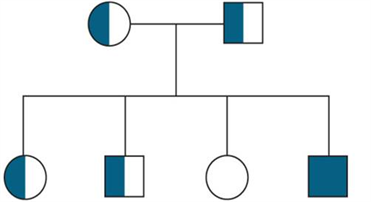
\includegraphics[width = \textwidth]{pedigree-diagram}\]


\section{Limitations of Mendelian genetics}
\label{sec:org547d672}

\subsection{First limitation}
\label{sec:org0613ca7}
Since chromosomes are the vehicles of Mendelian Genetics, a potential problem arises when there are many more traits that we may want to analyse than there are the number of chromosomes.
\\[0pt]

For example, humans have 23 pairs of chromosomes, but we certainly have more than 23 traits that can be studied. If several genes of different traits are located close to each other on the same chromosome, they will not segregate randomly, but will remain "linked" in descendent generations. Di- or multi-hybrid analysis of Mendelian genetics will get us nowhere.

\subsection{Second limitation}
\label{sec:orgec014d8}
Often, the expression of the phenotype is not straightforward, and cannot be analysed by Mendelian genetics. The following are some complicating factors of such phenotypes:

\subsubsection{Continuous variation}
\label{sec:org77612a2}
The continuous variation shown in some traits, like skin colour. The characters can show a range of small differences when multiple genes act jointly to influence a character.

\subsubsection{Pleiotropic effects}
\label{sec:org33090c2}
An allele that has more than one effect on a phenotype is considered pleiotropic. Mendelian genetics cannot handle this type of alleles because it is not clear-cut.

\subsubsection{Incomplete dominance}
\label{sec:org8d41b5e}
Not all alternative alleles are either fully dominant or fully recessive in heterozygotes. This complicates Mendelian genetic analysis.

\subsubsection{Environmental effects}
\label{sec:orgd005c43}
The degree to which many alleles are expressed depends on the environment.

\subsubsection{Codominance}
\label{sec:orgd4acd29}
A gene may have more than two alleles in a population, a few of which are dominant. For example, the ABO blood type. A and B alleles are both dominant.


\section{Molecular evidence for evolution}
\label{sec:org174872e}
All living organisms use the same basic biochemical molecules, utilise the same DNA triple code (codon), and utilise the same 20 amino acids in their proteins.
\\[0pt]

Very similar DNA sequences suggests recent common descent, while vastly different DNA base-sequences suggest a more ancient common descent.


\section{Other tools in molecular biotechnology}
\label{sec:orgf4bc0a5}

\subsection{Gel electrophoresis}
\label{sec:org79e660b}
Gel electrophoresis a method of separating and visualising DNA fragments. Running the DNA samples through the cell will allow the DNA samples to be separated by sizes. Those with the same size will end in the same band of the gel, which can be visualised by staining.

\subsection{DNA sequencing techniques}
\label{sec:orgaa07f24}
DNA sequencing techniques help to determine DNA sequences.

\subsection{Bioinformatics}
\label{sec:orgcbfb28b}
Bioinformatics is the management of biological information, such as a DNA sequence and protein sequence using a computer.

\subsection{Various ways to introduce manipulated DNA into cells}
\label{sec:orgb948fb8}
Some examples of such ways are:
\begin{itemize}
\item Transformation
\item Transfection
\item Microinjection
\end{itemize}

\newpage

\section{Molecular biotechnology in agriculture}
\label{sec:org79ac129}
Molecular biotechnology is applied in agriculture and an example is the engineering of crops to be resistant to insect pests. This reduces the need to add insecticides to the environment. For example, genes from the soil bacterium \emph{Bacillus thuringiensis} (Bt), which produces a protein that is toxic when eaten by crop pests, have been inserted into the chromosomes of tomatoes. The plant can now synthesise Bt protein, which are toxic to pests, such as the tomato horn worm.
\\[0pt]

Herbicide resistance has also been genetically engineered. Glyphosate is a powerful herbicide that kills most actively growing plants and is used to control weeds. Using a gene gun, engineers inserted an isolated gene from a bacterium that is resistant to glyphosate into crop plants. The glyphosate can now be widely applied to fields and orchards where it retards weed growth but not crop growth.
\\[0pt]

However, there are some concerns with transgenic crop plants, which are known as genetically modified (GM) crops. While there are benefits like soil preservation and reduced pesticide usage, there are also concerns over the use of GM food, such as:
\begin{itemize}
\item Is eating GM food dangerous? Foreign genes may introduce proteins that may be harmful when consumed and cause allergic reactions in some people.
\item Are GM crops harmful to the environment?
\begin{itemize}
\item There is a possibility of unintentional harm to other organisms. For example, weeds might be important sources of food and shelter for non-pest insects.
\item There is potential for new resistance. For example, pests might be likely to become resistant to the engineered proteins. Farmers are then required to plant some non-GM crop alongside the GM crop in order to slow the selection pressure for resistance.
\item Gene flow into neighbouring plants. For example, modified genes may spread to non-GM species due to interbreeding.
\end{itemize}
\end{itemize}


\section{Reproductive cloning}
\label{sec:orgcf98064}
\begin{itemize}
\item Reproductive cloning was proposed by Han Spemann in 1938, by removing the nucleus from an egg cell (called enucleated egg) and replacing it with a nucleus from a diploid somatic cell.
\item Attempts at cloning were made many years later by several researchers. Some success was obtained, but only with a donor nucleus from an embryo, not an adult nucleus.
\item Wilmut used an adult sheep's mammary gland as the nuclear donor, which ended up with "Dolly", who was born on July 5, 1996.
\item A wide variety of farm animals have been cloned since "Dolly" the sheep.
\item Cloning procedures have become increasingly efficient.
\item However, most cloned animals do not live a normal lifespan.
\end{itemize}

\subsection{Wilmut's animal cloning experiment}
\label{sec:orgde314e1}
\begin{enumerate}
\item Mammary cells are extracted and grown in nutrient deficient solution that arrest the cell cycle.
\item An egg cell is extracted from another animal.
\item The nucleus of the egg cell is removed with a micropipette. The egg is now left without a nucleus, which is a state known as enucleated.
\item The mammary cell is then inserted inside the covering of the egg cell.
\item An electric shock is applied which opens the cell membrane and triggers cell division.
\item With the initiation of cell division in vitro, the cell eventually develops into the embryo state.
\item The embryo is now ready to be implanted in a surrogate mother.
\item Within the womb, the embryo continues to develop.
\item After a five-month pregnancy, a lamb genetically identical to the sheep from which the mammary cell was extracted is born.
\end{enumerate}
\end{document}